\documentclass[11pt]{article}

%\documentclass[aoas,preprint]{imsart}

%\RequirePackage[OT1]{fontenc}
%\RequirePackage{amsthm,amsmath,amssymb,caption,graphicx,subcaption}
%\RequirePackage{natbib}
%\RequirePackage[colorlinks,citecolor=blue,urlcolor=blue]{hyperref}





\usepackage{algorithm, alltt, amssymb, amsfonts, amsmath, caption, color,
    fancyhdr, graphicx, mathrsfs, moreverb, natbib, setspace, subcaption, tikz,
    titling, ulem, verbatim}
\usepackage[noend]{algpseudocode}
\renewcommand{\algorithmicrequire}{\textbf{Input:}}
\renewcommand{\algorithmicensure}{\textbf{Output:}}

\addtolength{\oddsidemargin}{-.875in}
\addtolength{\evensidemargin}{-.875in}
\addtolength{\textwidth}{1.75in}
\addtolength{\topmargin}{-.875in}
\addtolength{\textheight}{1.75in}

\newtheorem{proposition}{Proposition}

\def\A{\mathcal A}\def\B{\mathcal B}\def\C{\mathcal C}\def\D{\mathcal D}
\def\E{\mathcal E}\def\F{\mathcal F}\def\G{\mathcal G}\def\I{\mathcal I}
\def\J{\mathcal J}\def\L{\mathcal L}\def\M{\mathcal M}\def\N{\mathcal N}
\def\O{\mathcal O}\def\P{\mathcal P}\def\Q{\mathcal Q}\def\R{\mathcal R}
\def\S{\mathcal S}\def\T{\mathcal T}\def\W{\mathcal W}\def\V{\mathcal V}
\def\X{\mathcal X}\def\Y{\mathcal Y}\def\Z{\mathcal Z}
\def\mI{\mathbb I}\def\mN{\mathbb N}\def\mP{\mathbb P}\def\mR{\mathbb R}
\def\mS{\mathbb S}
\def\bE{{\bf E}}
\def\bx{{\bf x}}

\def\bam{\hspace{1cm}$\blacksquare$}\def\pow{\hspace{1cm}\blacksquare}
\def\prob{\mbox{\bf prob}}\def\tr{\mbox{\bf tr}}
\def\l{\left}\def\r{\right}\def\lf{\lfloor}\def\rf{\rfloor}
\def\un{\underline}
\def\theat{\theta}\def\lambad{\lambda}\def\lamda{\lambda}
\def\minimize{\mbox{minimize}\hspace{4mm}}
\def\maximize{\mbox{maximize}\hspace{4mm}}
\def\subjectto{\mbox{subject to}\hspace{4mm}}
\def\iid{\stackrel{\mbox{\scriptsize i.i.d.}}{\sim}}

\title{True wOBA: Estimation of true talent level for batters}
\author{Scott Powers and Eli Shayer}

\begin{document}

\maketitle

\section{Introduction}
\label{sec-intro}

We begin with a thought exercise. Which statistic is more volatile:
on-base percentage (OBP) or batting average on balls in play (BABIP)? To
sharpen the question mathematically, suppose we observe the following data for
batter $B$:
\begin{itemize}
    \item $OBP_1$, his OBP in his first 150 plate appearances;
    \item $BABIP_1$, his BABIP on his first 150 {\it balls in play};
    \item $OBP_2$, his OBP in his second 150 plate appearances; and
    \item $BABIP_2$, his BABIP on his second 150 balls in play.
\end{itemize}
Which do you expect to be closer: $OBP_1$ to $OBP_2$, or $BABIP_1$ to
$BABIP_2$? In other words, which is a better predictor of itself: OBP or BABIP?
On the one hand, OBP is the statistic made famous by {\it Moneyball} for its
merits in player evaluation. On the other hand we have the notoriously
``luck-driven'' statistic BABIP. We know that OBP stabilizes at 460 plate
appearances while BABIP stabilizes at 820 balls in play \citep{Carleton12}.

The answer? {\it On-base percentage is more volatile}. When using $OBP_1$ to
predict $OBP_2$, the root mean square error (RMSE) is .062. When using
$BABIP_1$ to predict $BABIP_2$, the RMSE is a hair smaller, at .058.
Mathematically, this makes perfect sense. The league average BABIP is .299, and
the league average OBP is .317. So the standard binomial assumption implies
that OBP should have slightly higher variance than BABIP. Variance is, after
all, another word for volatility. To reiterate, {\it on average, observed BABIP
is just as close to true talent as observed OBP is, and possibly closer}.

Why, then, does BABIP get a bad reputation? It has to do with the definition
of stabilization rate, which is based on the number of trials needed from each
player in two different samples in order for the correlation between the two
estimates of the statistic (one from each sample) to exceed some threshold.
Under the assumption that observed OBP is equal to true talent plus noise,
we have
$$OBP_1 = OBP_{\mbox{\scriptsize true}} + \epsilon_1,\hspace{1cm}\mbox{and}
\hspace{1cm} OBP_2 = OBP_{\mbox{\scriptsize true}} + \epsilon_2,$$
where $\epsilon_1$ and $\epsilon_2$ are independent and identically
distributed, say with variance $\sigma^2_{\epsilon, \mbox{\tiny OBP}}$.
If the population variance in OBP true talent is
$\sigma^2_{\mbox{\tiny pop,OBP}}$, then
$$\rho_{\mbox{\tiny OBP}} \equiv \mbox{Corr}(OBP_1, OBP_2) =
    \frac{\mbox{Cov}(OBP_1, OBP_2)}
    {\sqrt{\mbox{Var}(OBP_1)\mbox{Var}(OBP_2)}} =
    \frac{\sigma^2_{\mbox{\tiny pop,OBP}}}
    {\sigma^2_{\mbox{\tiny pop,OBP}} + \sigma^2_{\epsilon,\mbox{\tiny OBP}}}$$

Similarly,
$$\rho_{\mbox{\tiny BABIP}} \equiv \mbox{Corr}(BABIP_1, BABIP_2) =
\frac{\sigma^2_{\mbox{\tiny pop,BABIP}}}
{\sigma^2_{\mbox{\tiny pop,BABIP}} + \sigma^2_{\epsilon,\mbox{\tiny BABIP}}}.$$
We have observed that
$\sigma^2_{\epsilon,\mbox{\tiny OBP}}$ is slightly larger than
$\sigma^2_{\epsilon,\mbox{\tiny BABIP}}$, so if
$\rho_{\mbox{\tiny OBP}} > \rho_{\mbox{\tiny BABIP}}$, then it must be
the case that $\sigma^2_{\mbox{\tiny pop,OBP}} >
\sigma^2_{\mbox{\tiny pop,BABIP}}$. Sure enough, this is exactly the case. Our
estimate of the population variance of OBP skill is about 33\% greater than our
estimate of the population variance of BABIP skill. So the slow stabilization
of BABIP is not driven by the volatility of the statistic but rather by the
lack of spread between players in the distribution of underlying true talent.
This is consistent
with the interpretation that BABIP has more to do with luck than does OBP,
because it means that there is less spread between good BABIP batters and bad
BABIP batters than there is between good OBP batters and bad OBP batters.

Because the spread in true talent BABIP is less than the spread in true talent
OBP, we can leverage this information to make even more accurate estimates of
BABIP using the technique of regression to the mean. We leave the details of
our implementation of regression to the mean to Appendix A of \citet{TheBook},
but it is a two-step procedure. In the first step, we estimate the underlying
true talent population variance of the statistic by comparing the observed
variance in the data to the theoretical variance if all players had equal
skill. In the second step, we take for each player a weighted average of the
population mean and his observed statistic, weighted by the inverse of the
population variance and the inverse of the statistic's sample variance,
respectively. This shrinkage of the estimates improves the RMSE of the OBP
estimator from .062 to .049 and improves the RMSE of the BABIP estimator from
.058 to .047. An important observation here is that correlation is not a good
measure of the accuracy of a prediction because of its scale invariance. For
example, the correlation of both the unregressed estimate of OBP and the
regressed estimate of OBP with the observed OBP in the second sample is 0.23.
The correlation is the exactly same for both estimators despite one being more
accurate than the other. For this reason, throughout the paper we use mean
square error (and RMSE) as our criterion for evaluating estimates.

\begin{table}[h]
\caption{\it Root mean square error for predicting the rate of each outcome
    using naive and regressed estimators. Each estimator uses the first 200 PAs
    for each batter to predict the rate at which that
    batter will produce the outcome in his second 200 PAs. The error is
    reported in percentage points, so for example the RMSE of 3.81 for the
    naive estimator of 1B rate corresponds to the difference between an
    estimate of 15.00\% and an observation of 18.81\%. The bottom row of the
    table gives the estimated population variance of the true talent for
    producing the corresponding outcome, in the same units (percentage points).}
\centering
\begin{tabular}{c|rrrrrrrrr}
% latex table generated in R 3.2.2 by xtable 1.8-0 package
% Mon Feb 01 19:52:33 2016
 & G & F & K & BB & HBP & 1B & 2B & 3B & HR \\ 
 \hline
 Naive error & 4.80 & 4.45 & 4.19 & 3.33 & 0.94 & 3.81 & 2.04 & 0.74 & 1.79 \\ 
  Regressed error & 4.42 & 4.22 & 3.89 & 3.04 & 0.80 & 3.17 & 1.62 & 0.67 & 1.61 \\ 
  \hline
  Population variance & 15.85 & 20.13 & 29.10 & 6.26 & 0.24 & 7.02 & 0.45 & 0.13 & 1.88 \\ 
  

\end{tabular}
\label{tab-rttm-by-event}
\end{table}

We apply the same methodology to the rates of each of nine different outcomes
of plate appearances, with the results presented in Table
\ref{tab-rttm-by-event}. Note that each outcome has a unique population
variance, with smaller population variances necessitating more aggressive
regression to the mean. Whereas strikeouts need very little regression to the
mean, doubles and triples should be regressed aggressively.

\begin{figure}[h]
\caption{\it Players plotted by mean-regressed wOBA vs. observed wOBA.
    Players with fewer than 50 PAs are orange dots, and players with at least 50
    PAs are blue circles. The horizontal dotted black line corresponds to
    league average wOBA, and the green diagonal line corresponds to True wOBA
    exactly equal to observed wOBA. We observe a steeper slope for the cloud
    of blue circles than for the cloud of orange dots because fewer PAs mean
    more aggressive regression to the mean.}
\centering
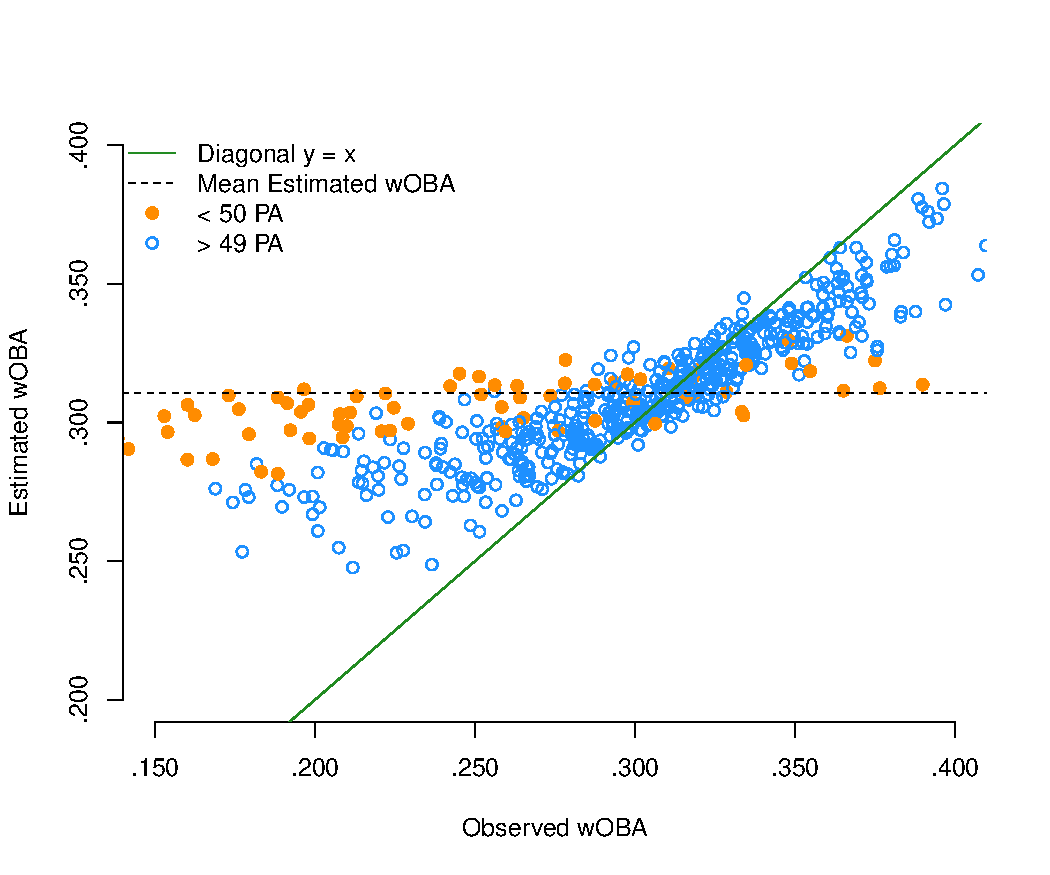
\includegraphics[width = 0.4\textwidth]{../figs/woba-observed-v-estimated.pdf}
\label{fig-woba-obs-v-est}
\end{figure}

We combine the regressed estimates summarized by Table \ref{tab-rttm-by-event}
to obtain a regressed estimate of wOBA for each batter based on his first 200
PAs. We plot regressed wOBA versus observed wOBA in Figure
\ref{fig-woba-obs-v-est}. The plot illustrates how players with relatively few
PAs are regressed further toward the mean than players with relatively many PAs.
Also, the players with the most extreme observed wOBAs take larger steps toward
the mean, reflecting that players with the best performances were likely lucky
in addition to being good.

\begin{figure}[h!]
\caption{\it Projected change in wOBA vs. observed BABIP. On the $y$-axis is
    regressed wOBA minus observed wOBA. The greater the
    BABIP, the lower the expected wOBA, relative to observed wOBA.}
\centering
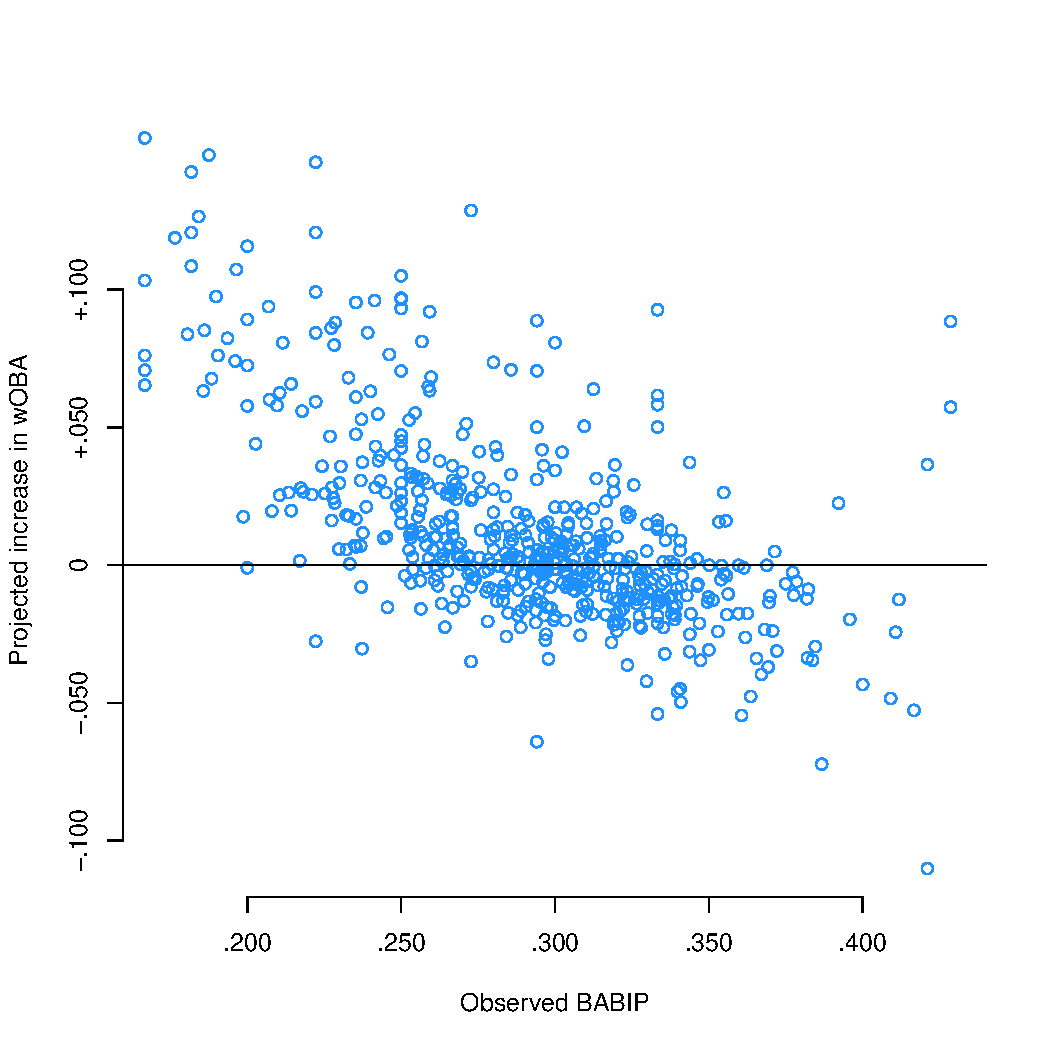
\includegraphics[width = 0.4\textwidth]{../figs/woba-v-babip.pdf}
\label{fig-woba-v-babip}
\end{figure}

Note that because we have differentially regressed the different outcome types,
less stable outcomes have been regressed more toward the mean than more stable
outcomes. Players with a high BABIP, for example, will be expected to have a
lower BABIP moving forward, according to this method. And in fact, Figure
\ref{fig-woba-v-babip} illustrates the relationship between observed BABIP and
the difference between observed wOBA and regressed wOBA. The higher BABIP is,
the lower regressed wOBA is relative to observed wOBA. This encapsulates and
precisely quantifies the common understanding that players with high BABIP
typically have been lucky and should expect their performance to drop.

Regression to the mean precisely quantifies claims that players with small
numbers of PAs or high BABIPs are unlikely to sustain their performance.
Moreover, it quantifies what performance we can expect moving forward.
In Section \ref{sec-methods} we connect regression to the mean with shrinkage
estimators in linear regression, thus extending the approach to account for
additional covariates and leading to the proposal of True wOBA. In Section
\ref{sec-results} we present the results of True wOBA on the 2015 MLB regular
season play-by-play data.


\section{Methods}
\label{sec-methods}

\subsection{Data}
\label{sub-data}

The dataset used throughout this paper is the 2015 Major League Baseball
regular season play-by-play dataset from Retrosheet. For each plate appearance
the data include, among other things, the identity ($B_i$) of the batter, the
identity ($P_i$) of the pitcher, the stadium ($S_i$) where the PA took place,
an indicator ($H_i$) of whether the batter was on the home team and an indicator
($O_i$) of whether the batter had opposite handedness from the pitcher.

For the present work, we consider only plate appearances which result in one of
the following outcomes: groundout (G), flyout (F), strikeout (K), base on balls
(BB), hit by pitch (HBP), single (1B), double (2B), triple (3B) or home run
(HR). If the batter reached base on an error, we count this as G or F depending
on the trajectory of the batted ball. We count all fielder's choices as G. We
discard intentional walks and catcher's interferences. We also discard PAs in
which the batter is a pitcher. The result is a dataset of 176,560 PAs featuring
660 unique batters and 735 unique pitchers.


\subsection{Regularization as regression to the mean}
\label{sub-regul-as-regre}

Suppose that batter $X$ has skill $\beta_X$ for hitting singles. Using $Y$ to
denote the outcome of a plate appearance for batter $X$, the probability model
defined by
$$\mP(Y = \mbox{1B}) = \frac{e^{\alpha + \beta_X}}{1+e^{\alpha + \beta_X}}$$
is a logistic regression model. The parameter $\alpha$ is an intercept term
corresponding to the baseline likelihood of a single. The larger
$\alpha + \beta_X$ is, the more likely it is that the PA results in a single.

More ambitiously, take $B_i$ to be the identity of the batter in the $i^{th}$
PA in the 2015 Retrosheet play-by-play data, for $i$ from 1 to 176,560. A model
which describes the distribution of all singles is given by:
\begin{equation}
\label{eqn-logistic}
\mP(Y_i = \mbox{1B}) =
    \frac{e^{\alpha + \beta_{B_i}}}{1+e^{\alpha + \beta_{B_i}}},
\end{equation}
independently for each $i$. Note that, for fixed intercept $\alpha$, this model
is identical to one in which each batter $X$ simply has some probability $p_X$
of hitting a single. This is due to the one-to-one correspondence between
$\beta_X$ and $p_X$.

To fit the model (\ref{eqn-logistic}), we seek to maximize its log-likelihood
$\ell(\beta|B, Y)$:
\begin{equation}
\label{eqn-loglike}
\max_\beta\ell(\beta|B, Y)
\equiv
\max_{\beta}\sum_{i=1}^{176560}\l\{Y_i\log\l(\frac{e^{\alpha+\beta_{B_i}}}
    {1+e^{\alpha+\beta_{B_i}}}\r) + (1-Y_i)\log\l(\frac{1}
    {1+e^{\alpha+\beta_{B_i}}}\r)\r\}
\end{equation}
which turns out to be equivalent to using the observed fraction of singles for
each batter as the estimate for his 1B rate. For example, a player who hit 15
singles in 100 PAs would be estimated to have a 1B rate of 15\%. We call this
the {\it naive} estimator of 1B rate. As discussed in Section \ref{sec-intro},
a batter estimator is the {\it regressed} estimator.

To relate our logistic regression model to regression to the mean, we appeal to
the concept of {\it regularization} from machine learning. Instead of solving
the optimization problem (\ref{eqn-loglike}), instead consider
\begin{equation}
\label{eqn-ridge}
\max_{\beta}\ell(\beta|B, Y) - \lambda\sum_{X \in \B}\beta_{X}^2.
\end{equation}
We have introduced a penaly parameter $\lambda > 0$, which is multiplied by
the sum of the squares of the skills of our set $\B$ of batters. To maximize
(\ref{eqn-ridge}), we must choose $\beta$ which explain the data well but are
also not too large, because we pay a penalty for $\beta$ which are far from
zero. The result is that the skill estimates $\beta_X$ are pulled toward zero,
and thus the estimates $p_X$ of 1B rate are pulled closer together, just as in
regression to the mean. The optimization problem (\ref{eqn-ridge}) is known as
ridge logistic regression, and we call the resulting estimator of 1B rate the
{\it ridge} estimator.

\begin{figure}[h]
\caption{\it Comparison of ridge estimator with regressed estimator of 1B rate.
    Batters with fewer than 20 PAs are orange dots, and batters with at least 20
    PAs are blue circles. The horizontal dotted black line corresponds to league
    average 1B rate. The diagonal green line corresponds to where the two
    estimators are equal. Figure (a) plots regressed estimates against naive
    estimates while figure (b) plots ridge estimates against naive estimates.
    The similarity of figures (a) and (b) suggests the close correspondence of
    the ridge and the regressed estimators, which is confirmed by figure (c),
    which plots regressed estimates against ridge estimates.}
\hspace{-1cm}
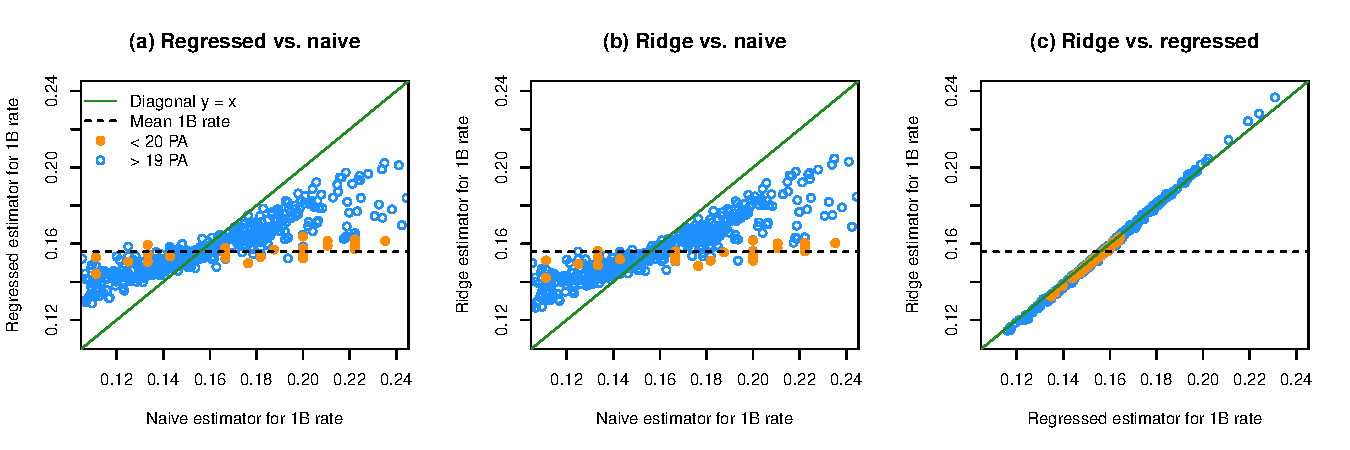
\includegraphics[width = 1.1\textwidth]{../figs/regul-as-regre.pdf}
\label{fig-regul-as-regre}
\end{figure}

The regularization parameter $\lambda$ is chosen through a process called cross
validation. We split the training data into 10 folds and for each fold, we use
the data not in that fold to predict the data in the fold, creating predictions
for many different values of $\lambda$. The value of $\lambda$ which leads to
the lowest error overall in the cross validation step is the one we use to fit
the model on the whole training set. Hence $\lambda$ is chosen with the goal of
minimizing prediction error in mind.

\begin{table}[h]
\centering
\caption{\it Root mean square error for predicting the rate of each outcome
    using naive, regressed and ridge estimators. Each estimator uses half of
    all plate appearance (selected at random) to predict the rate at which each
    batter will produce each outcome in the other half of the data. Error is
    evaluated on all players with at least 30 PAs in the held-out test set, and
    the error for each player is given weight proportional to his number of PAs
    in the held-out test set.}
\begin{tabular}{c|ccccccccc}
Estimator & G & F & K & BB & HBP & 1B & 2B & 3B & HR\\
\hline
% latex table generated in R 3.1.2 by xtable 1.7-4 package
% Mon Feb  1 17:05:34 2016
 Naive & 4.41 & 4.45 & 4.25 & 2.60 & 1.04 & 3.66 & 2.21 & 0.82 & 1.71 \\ 
  Regressed & 3.98 & 3.97 & 3.89 & 2.38 & 0.89 & 3.09 & 1.68 & 0.63 & 1.52 \\ 
  Ridge & 3.97 & 3.99 & 3.90 & 2.39 & 0.88 & 3.08 & 1.67 & 0.64 & 1.51 \\ 
  
\end{tabular}
\label{tab-regul-as-regre}
\end{table}

Conceptually, the ridge estimator is similar to the regressed estimator because
both apply a shrinkage to pull estimates of 1B rate toward a center. The
similarity between the two estimators is illustrated by Figure
\ref{fig-regul-as-regre}, which shows that the two estimators give nearly
identical results on the play-by-play data. Table \ref{tab-regul-as-regre}
demonstrates that this relationship extends beyond only 1Bs to cover all of the
other PA outcomes, as well. For each PA outcome, the ridge estimator leads to
an improvement in prediction over the naive estimator, yielding similar results
to the regressed estimator.

The key difference between the regressed estimator and the ridge estimator is
how each method determines how aggressively to shrink the results toward the
mean. The amount of shrinkage in regression to the mean is determined by the
population variance parameter, which itself is estimated by comparing observed
variance in the data to theoretical variance in binomial random variables, as
described in Section \ref{sec-intro}. The amount of shrinkage for the ridge
estimator, on the other hand, is determined by the regularization parameter
$\lambda$. The larger it is, the more aggressively estimates are regressed
toward their mean. Using cross validation to choose $\lambda$ means that we
are choosing the amount of shrinkage to minimize prediction error. This
approach directly attacks our goal of minimizing prediction instead of
estimating population variance as an intermediate step.

The bottom line is that instead of using regression to the mean, we can fit a
ridge logistic regression model and get similar
results. The advantage of this is that the logistic regression model can be
generalized to simultaneously adjust for park effects, opponent quality and
other factors. This upshot is the key idea behind our proposal, True wOBA.

\subsection{True wOBA}

For each outcome $k \in \{\mbox{G, F, K, BB, HBP, 1B, 2B, 3B, HR}\}$, the True
wOBA model is
\begin{equation}
\label{eqn-true-woba}
\mP(Y_i = k) = \frac{e^{\alpha_k + \beta_{B_ik} + \gamma_{P_ik} +
    \delta_{S_ik} + \zeta_kH_i + \theta_kO_i}}{1 + e^{\alpha_k + \beta_{B_ik} +
    \gamma_{P_ik} + \delta_{S_ik} + \zeta_kH_i + \theta_kO_i}}.
\end{equation}
As in Section \ref{sub-regul-as-regre}, this is a logistic regression model for
each outcome, but here it depends not only on the batter but also on the
pitcher and other variables. Refer to Section \ref{sub-data} for a description
of the data $B_i$, $P_i$, $S_i$, $H_i$ and $O_i$. The fixed, unknown paramaters
in (\ref{eqn-true-woba}) have the following interpretation:
\begin{itemize}
\item $\alpha_k$: the baseline log-odds of outcome $k$;
\item $\beta_{B_ik}$: the tendency of batter $B_i$ to produce outcome $k$;
\item $\gamma_{P_ik}$: the tendency of pitcher $P_i$ to produce outcome $k$;
\item $\delta_{S_ik}$: the tendency of stadium $S_i$ to produce outcome $k$;
\item $\zeta_k$: the increase in log-odds of outcome $k$ due to home field
    advantage; and
\item $\theta_k$: the increase in log-odds of $k$ due to the batter
    having opposite handedness from the pitcher.
\end{itemize}

True wOBA models the likelihood of an outcome as a tradeoff between the
batter's skill in producing the outcome and the pitcher's skill in preventing
it, with park effects and other adjustments built in. To fit each logistic
regression model we use ridge regression as in (\ref{eqn-ridge}). Because of
this ridge penalty, by construction the average batter has $\beta_{Bk} = 0$.
Similarly, the average pitcher has $\gamma_{Pk} = 0$, and the average stadium
has $\delta_{Sk} = 0$. We use the R package {\tt glmnet} \citep{glmnet} to fit
the ridge logistic regression (with 10-fold cross validation to choose
$\lambda$), yielding estimated coefficients $\alpha_k^*$, $\zeta_k^*$,
$\theta_k^*$, $\beta_{Bk}^*$ for each batter $B$, $\gamma_{Pk}^*$ for each
pitcher $P$, and $\delta_{Sk}^*$ for each stadium $S$.

For each batter $B$, the corresponding estimate of the probability that he
produces outcome $k$ in a plate appearance against an average pitcher in an
average stadium is given by
$$p_{Bk}^* = \frac{e^{\alpha_k^* + \beta_{Bk}^* + \zeta_k^*/2 + \theta_k^*/2}}
    {1 + e^{\alpha_k^* + \beta_{Bk}^* + \zeta_k^*/2 + \theta_k^*/2}}.$$
By using $\zeta_k^*/2$, this formulation mediates the two possibilities that
the batter is home or away. Similarly, using $\theta_k^*/2$ mediates the two
possibilities that the batter has opposite or same handedness as the pitcher.
Given $p_{Bk}^*$ for each batter $B$ and outcome $k$, we combine these
estimates into True wOBA using the wOBA weights published by FanGraphs
\citep{wOBAweights}.

For each pitcher $P$, the probability that he produced outcome $k$ when facing
an average batter in an average stadium is given by
$$p_{Pk}^* = \frac{e^{\alpha_k^* + \gamma_{Pk}^* + \zeta_k^*/2 + \theta_k^*/2}}
    {1 + e^{\alpha_k^* + \gamma_{Pk}^* + \zeta_k^*/2 + \theta_k^*/2}}.$$
We combine these estimated probabilities using the wOBA weights to get True
wOBA against for pitchers.

\subsection{Related work}

Several recent papers \citep{Brown08, Null09, Neal.etal10, Albert15} have
proposed methods for estimating or predicting batting statistics. In contrast
with projection systems, these methods implicitly assume that players' skills
remain constant between training sample and test sample (as opposed to
modeling the aging of skills). True wOBA differs from the above by adjusting
for park effects and quality of opposition.

A similar model which merits further discussion is Deserved Run Average
\citep[DRA]{Judge15}. At the core of DRA is a
regression model very similar to (\ref{eqn-true-woba}) which models the
distribution of outcomes as a function of the tradeoff between the batter's and
pitcher's skills, along with a plethora of control variables. This DRA model is
much more complicated than True wOBA, including, for example, adjustments for
the
identity of the umpire, game time temperature and a home field advantage that
varies by innning. Stripping the DRA model down to only the variables that True
wOBA uses to facilitate comparison, a light version of this core piece of DRA
models the wOBA on $i^{th}$ plate appearance as
$$\mbox{wOBA}_i = \alpha + \beta_{B_i} + \gamma_{P_i} + \delta_{S_i} + \zeta_kH_i + \theta_kO_i + \epsilon_i\mbox{, where}$$
\begin{equation}
\label{eqn-mixed}
\beta_B \iid \N(0, \sigma^2_\beta),\hspace{1cm}
    \gamma_P \iid \N(0, \sigma^2_P),\hspace{.5cm}\mbox{ and }\hspace{.5cm}
    \epsilon_i \iid \N(0, \sigma^2_\epsilon).
\end{equation}
So the batter skill paramaters $\beta_B$ are not fixed but random, with a
zero-mean normal distribution. Similarly, the pitcher skill parameters
$\gamma_P$ are random with a zero-mean normal distribution. The error terms
$\epsilon_i$ are standard in linear regression. All other parameters, including
the variance parameters $\sigma^2_\beta$, $\sigma^2_P$ and $\sigma^2_\epsilon$,
are fixed and unknown. This is called a mixed effects linear model because it
has both random and fixed parameters. It is fit via restricted maximum
likelihood, which will we do using the R package {\tt lme4} \cite{lme4}.

By assuming that the $\beta_B$ and the $\gamma_P$ come from a mean-zero
distribution, the mixed effects model (\ref{eqn-mixed}) shrinks its estimates
of the $\beta_B$ and $\gamma_P$ toward zero just as True wOBA does. This
connection is discussed in more detail in Section \ref{sub-regul-vs-rando}. The
key take-away from this section is that True wOBA is similar to a light version
of the core component of DRA. We compare this light version of DRA to True wOBA
in Section \ref{sub-validation}, under the name ``mixed effects model.''

\subsection{Regularization vs. random effect modelling}
\label{sub-regul-vs-rando}

We have two ways of achieving shrinkage of regression coefficient estimates:
regularization as in (\ref{eqn-ridge}) and random effect modelling as in
(\ref{eqn-mixed}). To facilitate comparison between the two approaches, we
introduce another wOBA estimator here based just on the identity of the batter,
as we did with the naive, regressed and ridge estimators from Section
\ref{sub-regul-as-regre}. We fit this model to each outcome category; for
example
\begin{equation}
\label{eqn-random}
\mP(Y_i = \mbox{1B}) = \Phi(\alpha + \beta_{B_i}),\hspace{1cm}
    \beta_B \iid \N(0, \sigma^2_B),
\end{equation}
where $\Phi(\cdot)$ is the standard normal cumulative density function. This is
probit regression, an alternative to logistic regression. Once we fit this
model using restricted maximum likelihood, for each batter $B$ we have
$\beta_B^*$, and the corresponding {\it random effect} estimator for the
probability that $B$ hits a single is $\Phi(\alpha^* + \beta_B^*)$. Table
\ref{tab-regul-vs-rando} compares the random effect estimator to the ridge
estimator in terms of test root mean square error after fitting each on a
randomly selected half of the play-by-play dataset. We observe that the two
estimators yield virtually identical results.

\begin{table}[h]
\centering
\caption{\it Root mean square error for predicting the rate of each outcome
    using ridge and random effect estimators. Each estimator uses half of
    all plate appearance (selected at random) to predict the rate at which each
    batter will produce each outcome in the other half of the data. Error is
    evaluated on all players with at least 30 PAs in the held-out test set, and
    the error for each player is given weight proportional to his number of PAs
    in the held-out test set.}
\begin{tabular}{c|ccccccccc}
Estimator & G & F & K & BB & HBP & 1B & 2B & 3B & HR\\
\hline
% latex table generated in R 3.1.2 by xtable 1.7-4 package
% Mon Feb  1 16:46:20 2016
 Regressed & 3.38 & 3.48 & 3.30 & 2.06 & 0.78 & 2.63 & 1.45 & 0.55 & 1.36 \\ 
  Random & 3.38 & 3.49 & 3.35 & 2.06 & 0.77 & 2.64 & 1.44 & 0.56 & 1.35 \\ 
  
\end{tabular}
\label{tab-regul-vs-rando}
\end{table}

The conceptual difference between the ridge estimator and the random effect
estimator is similar to the difference between the ridge estimator and the
regressed estimator. Like the regressed estimator, restricted maximum
likelihood for the random effect estimator uses the variance observed in the
response, relative to the expected variance if all players had the same
abilities, to infer the population variance of player's abilities. In that
sense the random effect model is a more direct extension of the regressed
estimator to allow for a linear model with covariates.

The ridge estimator has the advantage over the random effect estimator that it
could be further extended to a multinomial regression model, jointly modeling
the outcome probabilities under the restriction that they must sum to one.
However, as {\tt glmnet} is currently set up, it does not allow for
different penalties to be applied to the regression coefficients for different
outcome categories in multinomial regression, making this extension an area for
future work.

Computationally, the ridge estimator could be faster or slower than the random
effect estimator, depending on the number of values of $\lambda$ searched over
in the cross validation step. In practice, we have not found a substantial
difference between the two approaches of regularization and mixed effect
modelling.




\section{Results}
\label{sec-results}


\subsection{Validation}
\label{sub-validation}

We randomly selected some PAs to set aside as a test set and used the remaining
PAs as a training set to fit four different wOBA estimators: naive
wOBA, regressed wOBA, True wOBA and the mixed effects model. As an added
wrinkle, the test
set was not chosen uniformly at random. We biased the selection so that PAs
which feature opposite-handed batters and pitchers have a 90\% chance of being
held out for the test set while PAs with same-handed batters and pitchers have
a 10\% chance of being held out for the test set. This change in circumstances
corresponds to what a player might face if he plays against tougher competition
or moves to a new home stadium. We expect True wOBA and the mixed effects model
to pick up on the changing circumstances and make better predictions than
regressed wOBA.

\begin{table}
\caption{\it Out-of-sample prediction error for four wOBA estimators. The error
    reported is mean square error when predicting wOBA for each player with at
    least 100 PAs in the test set. The error for the prediction of each player
    is weighted according to how many PAs he has in the test set. The bottom
    row responds the standard error of our estimated mean square error. The
    error for True wOBA, in bold, is the lowest of all four.}
\centering
\begin{tabular}{c|rrrr}
Estimator           &  Naive    & Regressed & True          & Mixed\\
\hline
Estimated MSE       & 0.00456   & 0.00220   & {\bf 0.00173} & 0.00180\\
Stadard error       &$\pm$0.00044&$\pm$0.00018&$\pm$0.00014 &$\pm$0.00015
\end{tabular}
\label{tab-validation}
\end{table}

The result of our biased sampling scheme is a training set of 93,868 PAs and a
test set of 82,692 PAs. We evaluate each method based on how its predicted wOBA
compares with observed wOBA for the 349 batters who have more than 100 PAs in
the test set. Table \ref{tab-validation} summarizes the results. True wOBA has
the best performance, with strong evidence that it is better than regressed
wOBA but only weak evidence that it is better than the mixed effects model.

We conclude that there is some value to True wOBA in terms of predicting
future wOBA in a changing landscape. But the power of True wOBA is in its
interpretation, which allows us to adjust performance for sample size and other
variables.


\subsection{True wOBA}

We estimated True wOBA for all batters and True wOBA against all pitchers based
on the full set of 176,560 plate appearances in the play-by-play dataset.
Figure \ref{fig-true-woba} shows the results. Players with fewer than 20 PAs
tend to lie close to the horizontal line at mean wOBA because they have not
demonstrated sufficient evidence that their true skill is any different from
the average player. Players with the largest numbers of PAs tend to lie closer
to the green diagonal line because there are sufficient data to more precisely
estimate their true talent levels.

\begin{figure}[h]
\centering
\caption{\it Players plotted by True wOBA vs. observed wOBA. Figure (a) shows
    wOBA for all batters while figure (b) shows wOBA against all pitchers.
    Players with fewer than 20 PAs are orange dots, and players with at least 20
    PAs are blue circles. The horizontal dotted black line corresponds to
    league average wOBA, and the green diagonal line corresponds to True wOBA
    exactly equal to observed wOBA.}
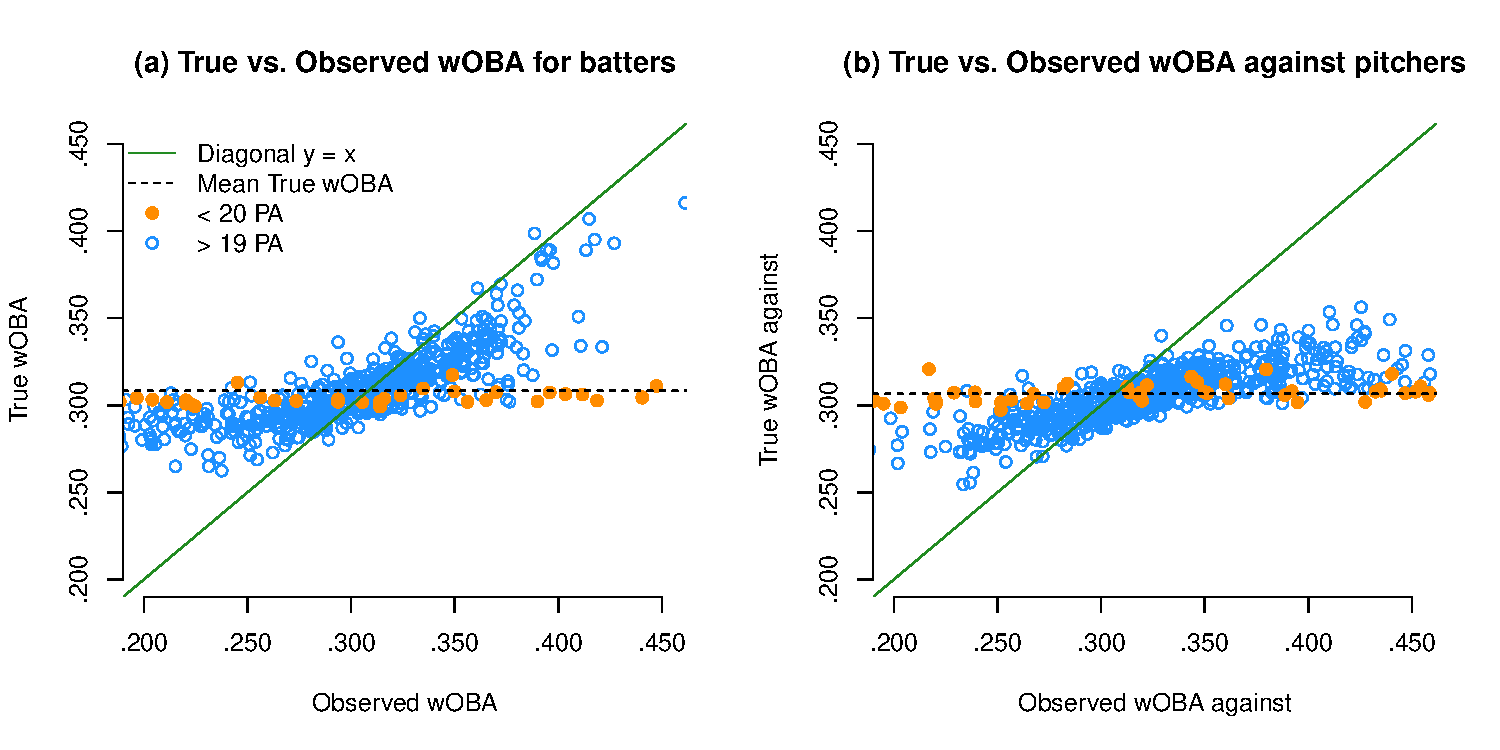
\includegraphics[width = .8\textwidth]{../figs/true-woba.pdf}
\label{fig-true-woba}
\end{figure}

We observe a steeper slope for the batters'
cloud of blue than for the pitchers' cloud of blue, reflecting more aggressive
regression to the mean for pitchers. This dovetails with the common
understanding in sabermetrics that pitchers have little control over the
results of balls in play. In other words, the population variance in true
talent level for outcomes on balls in play is relatively small for pitchers, so
it makes sense to regress their results more aggressively.

\begin{table}[h]
\caption{\it Leaders and laggards. This table lists the top 5 and bottom 5
    batters by True wOBA, as well as the top 5 and bottom 5 pitchers by True
    wOBA against.}
\centering
\footnotesize
\begin{tabular}{cccc||ccc}
&Batter             &Team& True wOBA & Pitcher      &Team& True wOBA against\\
\hline
&Bryce Harper       &WSN & .416 & Jake Arrieta      &CHC & .255\\
Top&Mike Trout      &LAA & .407 & Clayton Kershaw   &LAD & .256\\
5&Jose Bautista     &TOR & .399 & Zach Greinke      &LAD & .261\\
&Paul Goldschmidt   &ARI & .395 & Wade Davis        &KCR & .267\\
&Joey Votto         &CIN & .393 & Dallas Keuchel    &HOU & .267\\
~\\
&Alexi Amarista     &SDP & .270 & Jeremy Guthrie    &KCR & .346\\
Bottom&Chris Owings &ARI & .269 & Matt Boyd         &DET & .346\\
5&Ren\'{e} Rivera   &TBR & .265 & David Holmberg    &CIN & .349\\
&Danny Santana      &MIN & .265 & Dustin McGowan    &PHI & .354\\
&Omar Infante       &KCR & .262 & Allen Webster     &ARI & .356
\end{tabular}
\label{tab-leaders}
\end{table}

Table \ref{tab-leaders} shows the top and bottom players by True wOBA and True
wOBA against. Most interestingly, consider the top three pitchers in MLB by
True wOBA against: Jake Arrieta, Clayton Kershaw and Zach Greinke. These three
were also the three candidates in a hotly contested 2015 NL Cy Young Award
race. True wOBA agrees with the voters that Arrieta was the most deserving of
the award, despite Kershaw being No. 1 by FIP-WAR and Greinke being No. 1 by
RA9-WAR \citep{FanGraphs}. True wOBA mediates FIP-WAR and RA9-WAR by regressing
results on balls in play aggressively (and optimally, in terms of out-of-sample
prediction) but not ignoring them altogether.

The leaderboard also features 2015 AL Cy Young Award winner Dallas Keuchel at
No. 5 by True wOBA allowed and 2015 NL MVP Bryce Harper at No. 1 by True wOBA.
Mike Trout is a close second behind Harper at No. 2.

\begin{table}[h]
\caption{\it Largest differences between True wOBA and observed wOBA, among
    qualified players (min. 500 PAs). For each player $\Delta$wOBA is equal to
    True wOBA minus observed wOBA. We list the top 5 gainers and top 5 losers
    among both batters and pitchers.}
\centering
\footnotesize
\begin{tabular}{cccc||ccc}
&Batter             &Team& $\Delta$wOBA& Pitcher   &Team&$\Delta$wOBA against\\
\hline
&Wilson Ramos       &WSN & +.022 & Chris Rusin      &COL &--.068\\
Top&Michael Taylor  &WSN & +.021 & Kyle Kendrick    &COL &--.062\\
5&Albert Pujols     &LAA & +.017 & Jerome Williams  &PHI &--.047\\
&Alcides Escobar    &KCR & +.016 & Matt Garza       &MIL &--.045\\
&Chris Owings       &ARI & +.014 & Kyle Lohse       &MIL &--.041\\
~\\
&Anthony Rizzo      &CHC &--.035 & Jacob deGrom     &NYM & +.016\\
Bottom&Nolan Arenado&COL &--.037 & Sonny Gray       &OAK & +.016\\
5&Charlie Blackmon  &COL &--.039 & Clayton Kershaw  &LAD & +.019\\
&Bryce Harper       &WSN &--.045 & Jake Arrieta     &CHC & +.021\\
&David Peralta      &ARI &--.046 & Zach Greinke     &LAD & +.023
\end{tabular}
\label{tab-delta}
\end{table}

Table \ref{tab-delta} shows the players whose True wOBA is most higher than
observed their wOBA and the players whose True wOBA is most lower than their
observed wOBA. For example Wilson Ramos has a True wOBA which is 22 points
higher than his observed wOBA. The primary drivers of the difference between
True and observed wOBA are sample size (and fluctuations like in BABIP), park
effects and quality of opposition. It is no surprise that Rockies pitchers
Chris Rusin and Kyle Kendrick benefit the most from using True wOBA instead of
observed wOBA in their evaluation. Similarly, Rockies batters Nolan Arenado and
Charlie Blackmon are among those who drop the most going from observed wOBA to
True wOBA. All of the pitchers in the bottom of Table \ref{tab-delta} had
stellar seasons, as did Harper. Their presence in the bottom of the table
reflects the idea that those who performed best probably outperformed their
true talent the most.

\section{Discussion}

Nominally, this is a paper introducing True wOBA, a wOBA estimator which
simultaneously accounts for sample size, park effects and quality of opposition
to facilitate comparisons between batters and between pitchers on a level
playing field. But there is little thirst in the sabermetric literature for
new batting metrics. The real contribution of this paper comes in
three parts.

First, we argue against the use of stabilization rates when interpreting small
sample sizes. For one matter, stabilization rates have more to do with the
population variance in true skill level than variance in the observed
statistic. For another, there is a spectrum of sample sizes, not just ``too
small'' and ``big enough,'' a nuance not addressed by stabilization rates. We
advocate the use of regression to the mean to precisely quantify the
uncertainty due to finite sample sizes. A feature of regression to the mean for
wOBA is that it automatically learns that the population variance for
underlying BABIP skill is relatively small, thus regressing BABIP more
aggressively toward the mean. So regressed wOBA quantifies the assertion that
we expect players with high BABIP to see their performance drop off more than
players with low BABIP.

Second, we discuss in detail the relationship between regression to the mean
and its extension to shrinkage regression estimators pioneered by
\citet{Judge15}. In particular, we relate the penalty parameter in regularized
regression to the population variance parameter in regression to the mean to
explore conceptually the fundamental difference between how much shrinkage is
applied in each estimator.

Third, we make a novel comparison between regularized linear regression and
random effects linear models. This comparison leads to a discussion of the
relative strengths and weakness of the two approaches.

The goal of this paper is to review the fundamental statistical concepts that
relate to evaluating players on a level playing field, accounting for sample
size and other factors. No statistic readily available from FanGraphs.com or
Baseball-Reference.com accomplishes this task, which should be the first step
in player evaluation, as opposed to squinting at sample sizes and BABIPs to
ascertain whether a player's performance level is ``sustainable.''




\bibliographystyle{apalike}
\bibliography{baseball}

\end{document}
